% 2004 年全国卷Ⅲ理科第 20 题：三棱锥立体几何图
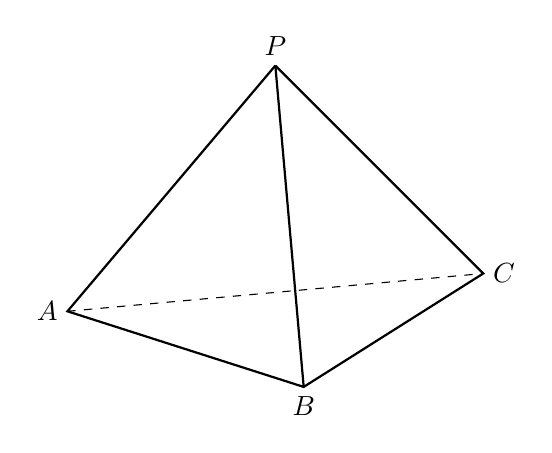
\begin{tikzpicture}[>=stealth,scale=1.2]
  % Coordinates
  \coordinate (A) at (-2.2,-0.4);
  \coordinate (B) at (0.3,-1.2);
  \coordinate (C) at (2.2,0);
  \coordinate (P) at (0,2.2);

  % Edges
  \draw[thick] (P) -- (A) -- (B) -- (C) -- (P);
  \draw[thick] (P) -- (B);
  \draw[dashed] (A) -- (C);

  % Labels
  \node[left] at (A) {$A$};
  \node[below] at (B) {$B$};
  \node[right] at (C) {$C$};
  \node[above] at (P) {$P$};
\end{tikzpicture}
